%% UVOD je posebej datoteka zaradi lažjega upravljanja.

\section{Uporaba računalnika v izobraževanju}
\label{sec:uporaba-raunalnika-v}

Model uporabe računalnika v izobraževanju je Gerlič \cite{gerlic_2000}
razdelil na tri področja.

\textbf{Primarno področje} lahko uvrstimo učenje programiranja, saj
sem prištevamo aktivnosti s katerimi želimo uporabnike seznaniti z
delovanjem in uporabo računalnika oz. sodobno informacijsko
komunikacijsko tehnologijo (\textbf{IKT})
\cite{model_uporabe_rac_izo-web}. Računalnik je tista učna vsebina, ki
jo obravnavamo.

\textbf{Sekundarno področje} sem spada vse tiste aktivnosti, katere so
vezane neposredno na izobraževalni proces katerega koli predmetnega
področja. Računalnik in \textbf{IKT} nastopata kot učno sredstvo ali
pripomoček v oblikah tradicionalnih računalniško podprtih učnih
sistemov ali inteligentnih ekspertnih sistemov.

\textbf{Terciarno področje}, spadajo vse aktivnosti, ki spremljajo
izobraževanje. Sem se štejejo aktivnosti izobraževanja, vodenja  in
upravljanja izobraževalnega sistema.

V tem diplomskem delu nas bo zanimalo le \textbf{primarno področje}
uporabe računalnika v izobraževanju, ki je razdeljeno v dveh pomembnih
področjih \cite{gerlic_2000}:

\begin{itemize}
\tightlist
\item kot element splošne izobrazbe,
\item kot element ožje strokovne - poklicne izobrazbe
  oz. usposabljanja.
\end{itemize}

\subsection{Splošnoizobraževalno področje}
\label{sec:spološnoiz_področje}

V današnjem času se računalnik kot element splošne izobrazbe kaže kot
velika potreba oz. se zdi znanje njegove uporabe samoumevno. Že pri
najmlajših otrocih računalnik vzbuja zanimanje in interes.  Računalnik
je postal intelektualno orodje in pripomoček v vsaki sferi človekove
dejavnosti in je prodrl tudi v šolo. Tako imenovana \textbf{računalniška
  pismenost} postaja nuja in zajema vse to kar bi človek moral znati o
računalniku in to, kako je potrebno z njim delati, da bo uspešno živel
v družbi, ki je osnovana na informacijah oz. informacijski družbi
\cite{klemencic_2011}.

V zvezi z definicijo in pojmovanjem \textbf{računalniške pismenosti}
se kažeta dve usmeritvi, Gerlič \cite{gerlic_2000} navaja številne
avtorje obeh usmeritev:

Prva poudarja \textbf{sposobnost računalniškega programiranj}a in
opredeljuje s pojmom pismenosti sposobnost branja in pisanja
podobno kot je to značilno za jezikovno pismenost. Tako zagovorniki,
te smeri poudarjajo, da je cilj računalniške pismenosti, učenje in
veščina programiranja z novim načinom mišljenja in strategijami
ugotavljanja in popravljanja računalniških programov.

Druga smer poudarja \textbf{splošno usposobljenost} za delo z
računalnikom in da ni smiselno, da vsak kdo postane programer, zaradi
tega, ker se bo računalnik uporabljal v najširšem smislu v
praksi. Pomembno za učenca je m da razume, delovanje računalnika in se
zaveda njegovega vpliva na razvoj družbe. Učencu moramo pomagati, da
dejanske probleme identificira in jih lahko reši že z narejeno
komercialno programsko opremo.

V zgodnjih letih sta bili značilni obe usmeritvi. Pozneje je prišlo do
preobrata leta 1987 po mednarodnem simpoziju na Univerzi v
Stanfordu. Eden od sklepov simpozija je bil ta, da se v
splošnoizobraževalne programe, ne uči več programiranja, še posebej ne
strukturiranih verzij programskega je na primer \textbf{BASIC}, temveč
naj se uči uslužnostne programske opreme, kot je urejevalnik besedil,
orodja za delo z podatkovnimi bazam, grafična grafična orodja itd..


%% Kje je programiranje, ali spada v strokovno izobraževanje in ne
%% spada v splošno računalniško pismenost, ali je danes zahteva po
%% zanju programiranju le to že uvrstila med splošno pismenost.

Ta dejstva je Gerlič \cite{gerlic_2000} povzel leta 2000 in je
predlagal isto usmeritev na: \emph{``Učencem vseh stopenj želimo ob
  čim večjem številu ur praktičnega dela z računalnikom, ob določenem
  problemu in ob uporabi ustreznih komercialnih programov seznaniti z
  osnovami računalništva in informatike.''} V nadaljevanju bomo lahko
ugotovili kakšni so današnji učni načrti za \textbf{OŠ} in \textbf{SŠ}
in ali so se zgornje ugotovitve uresničile in ohranile.

%%Moje misli.
Zanimivo bi bilo preiskati tudi kakšni so trendi danes? Ali zaradi
boljše računalniške pismenosti, predvsem mlajših generacij obstaja
potreba in trend, da se programiranje ponudi v širšem kontekstu tudi
na splošnem izobraževalnem nivoju.  Zanima nas koliko je računalniške
znanosti in programiranja v splošnoizobraževalnem področju, saj želimo
pokazati, da spletni portali za učenje programiranja zaradi
tehnološkega napredka omogočajo lažjo pot k učenju programiranja. Zato
nas po pozneje zanimalo kje je umeščeno v učnem načrtu programiranje v
\textbf{OŠ} in \textbf{SŠ}.

%% Podrobneje kje se izvaja računalniško izobraževanje v OŠ in SŠ
%% imamo v posebej zato namenjenem poglavju Računalništvo se ne izvaja
%% kot redni predmet, temveč poteka v

\subsection{Strokovno izobraževalno področje}
\label{sec:strokovno_izo_področje}

%% Gerlič 2000 -> ima večji del tega poglavja namenjenega znanje
%% računalništva za pedagoške delavce.

Sem prištevamo vse tiste aktivnosti, s katerimi želimo udeležence
izobraževanja usposobiti na različnih ravneh tako, da se bodo ti z
računalnikom in informacijskimi sistemi ukvarjali na poklicni ravni
\cite{gerlic_2000}.

%%Tu sem napisal po svoje.
Gerlič raziskuje podrobno strokovno področje na katerem se
izobražujejo bodoči učitelji računalništva. Lahko povemo, da sem
spadajo vse ozko usmerjene računalniške in informacijske smeri srednjih
šol, visokih ter univerzitetnih študijev. Zanima nas področje
programiranja, kar je predvsem predmet strokovnega
izobraževanja. Čeprav se bomo v diplomskem delu posvetili spletnim
portalom za učenje programiranja na splošnem nivoju, bomo pozneje vso
znanje zlahka prenesli tudi na ožje strokovno izobraževanj, saj je tu
uvod, začetkov programiranja, podoben na vseh težavnih stopnjah.

\subsection{Programiranje v OŠ}
\label{sec:Programiranje_v_OŠ}

Pouk računalništva v OŠ poteka kot izbirni predmet ali kot neobvezni
izbirni predmet. Za začetek bomo navedli kako je definirano
Računalništvo v učnem načrtu za izbirne predmete v osnovni šoli
\cite{ucni_nacrt-izbirni-os}:
\emph{``Računalništvo je
  naravoslovno-tehnični izbirni predmet, pri katerem se spoznavanje in
  razumevanje osnovnih zakonitosti računalništva prepleta z metodami
  neposrednega dela z računalniki, kar odpira učencem in učenkam
  možnost, da pridobijo tista temeljna znanja računalniške pismenosti,
  ki so potrebna pri nadaljnjem izobraževanju in vsakdanjem življenju.
  ''}.

\subsubsection{Izbirni predmet računalništva}
\label{sec:izbirni_predmet_rac}

Izbirni predmeti računalništva so sestavljenih z treh predmetov in jih
učenke in učenci lahko izberejo v tretjem trilerju, v 7., 8. in/ali
9. razredu. Prvi od teh predmetov je \textbf{računalništvo - urejanje
  besedil}, kjer si učenci pridobijo osnovna znanja, ki so potrebna za
razumevanje in temeljno uporabo računalnika. Naslednja dva predmeta
sta \textbf{računalniška omrežja} in \textbf{multimedija}, kjer se ta
znanja spiralno nadgradijo.

%Koliko ur je posamezen izbirni predmet

Zanima nas kje se pri teh predmetih računalništva pojavlja
programiranje. Vsak izmed teh predmetov ima operativne učne cilje tako
razdeljeno, da programiranje najdemo v tretji enoti, ki spada med
dodatne vsebine. Posamezne operativne cilje, dejavnosti in vsebino
prikazuje tabela \ref{tab:cilji_izb_prog}.

\begin{table}[!htb]
  \caption{Operativni cilji, dejavnosti in vsebine izbirnega predmeta
    računalništvo za III. dodatno enoto. \cite{ucni_nacrt-izbirni-os}}.
\label{tab:cilji_izb_prog}
\begin{tabular}{
  | p{0.33\linewidth-2\tabcolsep} |
  p{0.33\linewidth-2\tabcolsep} |
  p{0.33\linewidth-2\tabcolsep} | }
  \hline
  \rowcolor{gray!50}
  \textbf{OPERATIVNI CILJI} & \textbf{DEJAVNOSTI} & \textbf{VSEBINE} \\
  \hline

  \begin{itemize}[leftmargin=*]
    \tightlist
  \item napisati algoritem z odločitvijo, ki reši preprost vsakdanji
    problem;
  \item izdelati in spremeniti računalniški program z odločitvijo.
  \end{itemize}
  &
  \begin{itemize}[leftmargin=*]
  \item analizirati preprost problem;
  \item uporabljati osnovne korake programiranja.
  \end{itemize}
 &
  \begin{itemize}[leftmargin=*]
  \item risanje diagrama poteka za problem z odločitvijo;
  \item izdelava računalniškega programa.
  \end{itemize}
 \\
 \hline

\end{tabular}
\end{table}

Programiranje se pojavlja le kot dodatna vsebine, kar se kaže v
uresničitvi smeri računalništva, ki zagovarja \textbf{splošno
  usposobljenost}, kot smo jo opredelili v poglavju
\ref{sec:spološnoiz_področje}. Vendar se tu učiteljem računalništva
ponuja izjemna priložnost, da z učenci in učenkami naredi korak v
osnove programiranja.

\subsubsection{Neobvezno izbirni predmet računalništva}
\label{sec:neobvezno_izbirni_predmet_rac}

Opredelitev predmeta v učnem načrtu
\cite{ucni_nacrt-neobvezni-izbirni-os}, pravi, da neobvezni izbirni
predmet računalništva učence seznanja z različnimi področji
računalništva, računalniškimi koncepti ter procesi in jih ne učijo
dela z posameznimi programi. Učenci se seznanjajo tehniko in metodami
reševanja problemov, razvijajo algoritmičen način
razmišljanja. Opredelitev zadostuje prvi smeri računalniške
pismenosti, ki zagovarja \textbf{sposobnost računalniškega
  programiranja.}. Ker se v tej diplomski nalogi še posebej posvečamo
programiranju nam učni načrt tega predmeta dosti bolj ustreza in si ga
bomo podrobneje pogledali, saj nam bo pregled operativnih ciljev
služil kot vodilo pri nadaljnjem delu.  Najprej preglejmo splošne
cilje, katere povzemamo po učenem načrtu
\cite{ucni_nacrt-neobvezni-izbirni-os} in jih morajo doseči učenci:
\begin{itemize}
\tightlist
\item spoznavajo temeljne koncepte računalništva,
\item razvijajo algoritmični način razmišljanja in spoznavajo
  strategije reševanja problemov,
\item razvijajo sposobnost in odgovornost za sodelovanje v skupini ter
  si krepijo pozitivno samopodobo,
\item pridobivajo sposobnost izbiranja najustreznejše poti za rešitev
  problema,
\item  spoznavajo omejitve človeških sposobnosti in umetne
  inteligence,
\item se zavedajo omejitev računalniških tehnologij,
\item pridobivajo zmožnost razdelitve problema na manjše probleme,
\item se seznanjajo z abstrakcijo oz. poenostavljanjem,
\item spoznavajo in razvijajo zmožnost modeliranja, strokovno
  terminologijo.
\item  razvijajo ustvarjalnost, natančnost in logično razmišljanje,
\item razvijajo in bogatijo svoj jezikovni zaklad ter skrbijo za
  pravilno slovensko izražanje in strokovno terminologijo.
\end{itemize}

Neobvezni izbirni predmet je namenjen učencem 4., 5. in 6. razreda. V
učnem načrtu so operativni cilji predstavljeni tako, da so temeljni
označeni \textbf{krepko} in izbirni \emph{poševno}. Navedli bomo
tiste, ki so navezujejo na programiranje in strategije reševanja
problemov. Operativni cilji so razdeljeni na vsebinske sklope.

\textbf{Vsebina/sklop: Algoritmi}
\begin{itemize}
\tightlist
\item \textbf{razumejo pojem algoritem},
\item \textbf{znajo vsakdanji problem opisati kot zaporedje korakov},
\item \textbf{znajo z algoritmom predstaviti preprosto opravilo},
\item \textbf{algoritem predstavijo simbolno (z diagramom poteka) ali s
  pomočjo navodil v preprostem jeziku},
\item \textbf{sledijo algoritmu, ki ga pripravi nekdo drug},
\item \textbf{znajo v algoritem vključiti vejitev (če) in ponavljanje (zanke)},
\item \emph{znajo algoritem razgraditi na gradnike (podprograme)},
\item \textbf{znajo povezati več algoritmov v celoto, ki reši neki problem},
\item \emph{razumejo vlogo testiranja algoritma in vedo, da je testiranje
  orodje za iskanje napak in ne za potrjevanje pravilnosti},
\item \emph{primerjajo več algoritmov za rešitev problema in znajo poiskati
  najustreznejšega glede na dana merila},
\item \emph{znajo uporabiti nekatere ključne algoritme za sortiranje in
  iskanje},
\item \emph{poznajo osnovne algoritme za iskanje podatkov}.
\end{itemize}

\textbf{Vsebina/sklop: Programi}
\begin{itemize}
\tightlist
\item \textbf{znajo slediti izvajanju tujega programa},
\item \textbf{znajo algoritem zapisati s programom},
\item \textbf{znajo v program vključiti konstante in spremenljivke},
\item \textbf{ razumejo različne podatkovne tipe in jih znajo uporabiti v
  programu},
\item \textbf{znajo spremenljivkam spremeniti vrednost s prireditvenim
  stavkom},
\item \textbf{znajo v programu prebrati vhodne podatke in jih vključiti v
  program},
\item \textbf{znajo izpisovati vrednosti spremenljivk med izvajanjem programa
  in izpisati končni rezultat},
\item \textbf{v program vključijo logične operatorje},
\item \textbf{znajo uporabiti pogojni stavek in izvesti vejitev},
\item \textbf{razumejo pojem zanke in ga znajo uporabiti za rešitev problema},
\item \emph{razumejo kompleksnejše tipe podatkov (nizi, seznami/tabele) in
  jih znajo uporabiti v programu},
\item \textbf{prepoznajo in znajo odpraviti napake v svojem programu},
\item \emph{znajo popraviti napako v tujem programu},
\item \emph{znajo spremeniti program, da dosežejo nov način delovanja
  programa},
\item \emph{znajo rezultate naloge zapisati v datoteko},
\item \textbf{se seznanijo z dogodkovnim programiranjem},
\item \textbf{so zmožni grafične predstavitve scene (velikost objektov, ozadje, pozicioniranje)},
\item \textbf{so zmožni sinhronizacije dialogov/zvokov},
\item \textbf{so zmožni razumeti in realizirati interakcije med liki in objekt}i,
\item \textbf{ so zmožni ustvarjanja animacij}.
\end{itemize}

\textbf{Vsebina/sklop: Podatki}
\begin{itemize}
\tightlist
\item \textbf{razlikujejo podatek in informacijo},
\item \textbf{razumejo dvojiški sistem zapisovanja različnih podatkov},
\item \textbf{razumejo kodiranje podatkov},
\item \textbf{razumejo, da obstajajo podatki v različnih pojavnih oblikah
  (besedilo, zvok, slike, video)},
\item \emph{poznajo načine predstavitev določenih podatkov in odnose med
  njimi (dvojiška drevesa in grafi)},
\item \emph{vedo za stiskanje podatkov in vedo, da je stiskanje lahko brez
  izgub ali z izgubami},
\item \textbf{pojasnijo razliko med konstantami in spremenljivkami v programu},
%\item \textbf{znajo strukturirane podatke zapisati v tabele z vrsticami in
  %stolpci},
%\item \textbf{opišejo potrebo po urejanju podatkov},
\item \emph{poznajo osnovne algoritme za iskanje podatkov},
%\item \textbf{se zavedajo pomembnosti varovanja osebnih podatkov}.
\end{itemize}

\textbf{Vsebina/sklop: Reševanje problemov}
\begin{itemize}
\tightlist
\item \emph{znajo uporabiti različne strategije za reševanje problema},
\item \textbf{znajo našteti faze procesa reševanja problema},
\item \emph{znajo postavljati vprašanja in ugotoviti, kateri podatki so
  znani},
\item \emph{znajo za podano nalogo izluščiti bistvo problema},
\item \textbf{znajo najti ustrezno orodje, s katerim rešijo problem},
\item \textbf{znajo problem razdeliti na več manjših problemov},
\item \textbf{znajo načrtovati in realizirati rešitev},
\item \emph{za podano rešitev znajo oceniti posledice in vpliv na ``okolje''},
\item \emph{znajo uporabiti znano strategijo v novih okoliščinah},
\item \emph{znajo ustvariti nov algoritem za bolj kompleksne probleme},
\item \textbf{znajo učinkovito sodelovati v skupini in rešiti problem
    z uporabo informacijsko-komunikacijske tehnologije znajo ceniti
    neuspešne poskuse reševanja problema kot del poti do rešitve},
\item \emph{znajo kritično ovrednotiti rešitev in ugotoviti ali rešitev
  uspešno reši dani problem},
\item \emph{znajo kritično ovrednotiti strategijo reševanja problema},
\item \emph{zavedajo se omejitev informacijsko-komunikacijske tehnologije
  pri reševanju problemov}.
\end{itemize}

\textbf{Vsebina/sklop: Komunikacija in storitve}
\begin{itemize}
\tightlist
%\item \textbf{poznajo temeljne ideje o delovanju računalniških omrežij},
%\item \textbf{poznajo glavne storitve računalniških omrežij (e-pošta, splet
  %idr.)},
\item \textbf{znajo uporabiti ustrezna orodja in metode za iskanje po spletu},
\item \textbf{znajo uporabiti različne iskalne strategije v iskalnikih},
\item \textbf{poznajo omejitve pri rabi na spletu najdenih informacij
  (zavedajo se pojma intelektualna lastnina)},
%\item \textbf{znajo prikazati podatke na ustrezen način},
%\item \textbf{poznajo glavna varnostna priporočila v omrežjih in omrežni
  %bonton (netetika)}.
\end{itemize}

Kot smo že povedali smo nekatere cilje izvzeli, čeprav je znanje
računalniških omrežij pomembno, ga z vidika programiranja lahko
izpustimo. Lahko povemo, da nam je večina operativnih ciljev ostala,
saj smo jih lahko izključili le malo. Pridemo do spoznanja, da se v
računalniški znanosti pretežen del znanja vrti okoli programiranja in
reševanja problemov. Z samih ciljev lahko spoznamo tudi samo
zahtevnost snovi. Lahko si upamo napovedati, da jih bomo s pravimi
orodji kot so spletni portali za učenje programiranj tudi lažje
dosegli.

\subsection{Programiranje v SŠ}
\label{sec:Programiranje_v_SŠ}

% Dobor bi bilo, da za programiranje SŠ povzamemo splošni program
% gimnazije. OŠ ima zelo zahtevne cilje, lahko bi jih povzeli in
% dodali noto težavnosti.

%Določiti moramo, kateri srednješolski program bomo povzeli.
%Predlagam, splošno gimnazijo z 4. letnim programom rac in informatika

Pregled: informatika - Gimnazija
Pregled: računalništvo - Tehnična gimnazija.

\section{Zgodovina programskih jezikov v izobraževanju}
\label{sec:zgodovina_programskih_jezikov}


%Splošna zgodovina uporabe računalništva v izobraževanju
%Razdeljeno imam zgodovino rac. v izobrazevanju in programiranje v
%izo, ali je naj vse skupaj. Na kratko dodaj računalniška obdobja, kot
%jih je predstavil Gerlič


Uporaba računalništva v izobraževanju je bila deležna številnih
sprememb. Sama uporaba računalnika v izobraževanju je tesno
povezana z razvojem računalnikov.  Začetno obdobje, 1960 letih
prejšnjega stoletja so računalniki bili zelo dragi in veliki glavni
računalniki ( \emph{ang. mainframe} ), na njih se je učilo
programiranja, a so se uporabljali tudi za druga področja.
//-\textgreater{} Terminalska obdobje, Poglej gerliča. V tem obdobju
se je za učenje programiranja uporabljal \textbf{FORTRAN} ali
\textbf{asembler}. Programi so bili majhi in enostavi, zaradi fizičnih
omejiteh takratnega delovnega pomnilnika.

V 1970 so na trg prišli manjši računalniki, ki so bili tudi cenejši in
zmogljivejši. V tem času pride v ospredje strukturirano programiranje.
Najpopularnejši programski jezik je bil \textbf{PASCAL}.

V 1980 so se prvič pojavili samostojni osebni računalniki. Programski
jeziki v tem obdobju so bili strukturirani in močnega tipa (
\emph{ang.  strong type.} ). Med te spada \textbf{Ada, Modul 2, ML in
  naj omenimo še Prolog}.

V naslednjem desetletji, 1990 so v ospredje
prišli objektno orjentirani programski jeziki, kot sta \textbf{JAVA}
in \textbf{C\#} \cite{thesisAWebP}.

% //Umestitev računalnik v izobraževanju na primarnem področju.
% -\textgreater{} Gerlič Uporaba računalika v namene učenje računalništva
% in programiranja.

% //Doodaj generacije programskih jezikov. //Dodaj vrste programskih
% jezikov.

Metode poučevanja računalništva so se prav tako spreminjale. 1960 so
računalnike uporabljali samo za poučevanje programiranja. Povdarek pri
predmetih programiranja je bil predvsem na detaljlih zmožnosti
programskega jezika. Programiranje je bilo omejeno le na reševanje
enostavnih primerov in povdarek ni bil na reševanju problemov na
splošno.

V 1970 je reševanje problemov in abstrakcija podatkov postala glavni
in najpomembnejši del vseh programerskih predmetov, kar velja še
danes.  Programi so postali večji, bolj interaktivni in spremenil se
je vnos podatkov z tekstovnega v grafičnega. Vsebina predmetov
računalništva se je hitro razširjala, kakor so se množili številni
programski jeziki \cite{thesisAWebP}.

% //Misel: V izobraževanju je potrebno previdno izbrati obseg in področja
% vsebin, pri čemer ne smemo zanemariti timsko delo.

%\section{Učenje programiranja}
%\label{sec:učenje_programiranja}

\section{Računalniška znanost in programiranje}
\label{sec:računalniška_znanost_in_programiranje}

Računalniška znanost ima številne različice definicij, v grobem jo
lahko definicijo strnemo v naslednjih trditvah \cite{guideTCS}.

\begin{itemize}
\tightlist
\item Ukvarja z značilnostmi tisktega kar je izračunljivo.
\item Je znanost, ki izhaja iz več podroćij in ime korenine v matematiki,
znanosti in inženirstvu.
\item Ima mnoga podpodročja in je interdisiplinarna z biologijo,
ekonomijo, medicino, zabavo.
\item Ime računalništvo ali računalniška znanost nas lahko tudi zavede in
jo zamenjamo z področjem uporabe računalnika.
\end{itemize}

%Še je potrebno dodati kakšno definicijo z druge literature.

\subsection{Osnovni pojmi}
\label{sec:kaj_je_programiranje}

%% Splošne definicije programiranja.
%% Ni le pisanje kode temveč tudi uspešno reševanje nalog in
%% problemov?

Preden nadaljujemo moramo razjasniti nekaj osnovnih pojmov, ki se
pojavljajo računalniški znanosti.

\subsubsection{Program}
\label{sec:program}

Računalniški program je zbirka navodil, ki opravlja točno določeno
nalogo in jo izvajamo na računalniku. \textbf{Centralno procesna
  enot}a je tista, ki izvajanje programa omogoča. Računalniški program
navadno napiše \textbf{programer} v nekem \textbf{programskem jeziku},
postopku pisanja programa pravimo \textbf{programiranje}. Programski
jezik omogoča, da je program zapisan v takšni obliki, da je berljiv za
ljudi in je zapisan v \textbf{izvorni kodi}. Da računalnik razume
napisan program, ga prevede \textbf{prevajalnik
  (\emph{ang. compiler})} v \textbf{strojno kodo.}
\cite{wiki:computer_program}.

\subsubsection{Algoritem}
\label{sec:algoritem}





\subsubsection{Programiranje in kodiranje}
\label{sec:programiranje_kodiranje}


\subsection{Programske paradigme}
\label{sec:programske_paradigme}

Paradigma je način kako obravnavamo in gledamo na stavri, je okvir v
katerem leži naša interpretacija realnosti sveta. Paradigma
najpogosteje pomeni vzorec delovanja v znanstvenem ali drugem
raziskovanju.  Izraz programske paradigme je več pomenka, ki povzema
mentalne procese, strategije reševanja problemov, povezave med
različnimi paradigmami, programske jezike, stil programiranja in še
več (Wikipedia: Paradigma) \cite{guideTCS}.

Povemo lahko, da je programiranja, hevristična paradigma za algoritme
ki rešujejo probleme. Programski jezik je način za izražanje
programske paradigme.

%//Glavna definicija.
Programske paradigme so hevristike, ki se uporabljajo za reševanje
problemov. Programska paradigma analizira problem, čez specifičen
pogled in na ta način formulira rešitev za dani problem, ki ga razdeli
na manjše dele med katerimi definira razmerja.

Programske paradigme so na primer proceduralno, objektno orientirano,
funkcijsko, logično in istočasno programiranje.

V nadaljevanju bomo spoznali značilnosti dveh programskih paradigem.

\subsubsection{Proceduralno programiranje}
\label{sec:proceduralno_programiranje}

\subsubsection{Objektno orientirano programiranje}
\label{sec:objektno_orijentirano_programiranje}

\subsection{Programski jeziki}
\label{sec:programski_jeziki}

\subsection{Osnovni koncepti programiranja}
\label{sec:Osnvni koncepti_programiranja}

% Predstavljeni koncepti na primerih eden OŠ Scratch drugi Python.
V naslednjem odstavku se bomo vprašali kako lahko formuliramo sintakso
programskega jezika? In kaj je npr. definicija \emph{kopice}.

V ta namen definiramo mehko idejo po avtorju Hazzan \cite{guideTCS},
ki je naslednja. Mehka ideja je koncept, ki mu ne moremo pripisati
toge, niti formalne definicije. Mehke ideje ni niti možno opisati z
točno določeno aplikacijo. Na tem mestu se postavlja vprašanje kako
lahko defineramo nekaj kar se odvija po korakih.

Da odgovorimo na zgornji dve vprašanji, lahko povemo, da so pravila
sintakse togi orisi pri pisanju programske kode in da so semantična
pravila mehke ideje. Opozorimo še na to, da koncepti v računalniški
znanosti niso le toga pravila ali samo mehke ideje, temeč skupek
obojega. V spodnji tabeli \ref{tab:koncept_spremenljivka} prikazuje
primer spremenljivke.


\begin{table}[!htb]

\caption{Prikaz dvojnih, togih in mehkih orisov idej na primeru
  spremenljivke \cite{guideTCS}. }
\label{tab:koncept_spremenljivka}
\begin{tabular}{
  | p{0.30\linewidth-2\tabcolsep} |
  p{0.30\linewidth-2\tabcolsep} |
  p{0.40\linewidth-2\tabcolsep} | }
  \hline
  \rowcolor{gray!50}
  & \textbf{togi orisi} & \textbf{mehki orisi}\\
  \hline
  ime spremenljivke & Pravilo sintakse. & Potreba po imenu
                                          spremenljivke. Katero ime
                                          spremenljivke je pomembno in
                                          zakaj ga je potrebno
                                          določiti.\\
  \hline
  vrednost spremenljivke & Pravila tipa spremenljivke. Rezervacija
                           pomnilnika. & Spremenljivka ima eno
                                         vrednost, ki se lahko
                                         spreminja s časom.\\
  \hline
  dodelitev začetne vrednosti & Pravila sintakse. & Pomen dodelitve
                                                  začetne vrednosti\\
  \hline

\end{tabular}
\end{table}


\section{Spletni portali za učenje programiranja}
\label{sec:SPUP}

Spletne portale za učenje programiranja (\textbf{SPUP}) bomo
predstavili in spoznali tako, da bomo najprej pregledali kaj so bili
glavni razlogi, da se je pojavili razvoj teh na univerzah, ki
poučujejo računalniško znanost. Razen tehnoloških zmožnosti IKT za
nastanek spletnega portala nas bodo zanimale težave, ki so jih skušali
premostiti z SPUP.

Spletni portali za učenje programiranja so nastali na različnih
univerzah po svetu. V nadaljevanju bomo pregledali nekaj takšnih
primerov. Zanimal na s po spletni portal, ki je nastal na \emph{odprti
univerzi v Hong Kong-u} (\textbf{OUHK}), na \emph{Univerze Strathclyde iz
Valike britanije} (\textbf{US}). %Dodaj še druge UNI!

Zanimali nas bodo predmeti, ki veljajo za začetne pri poučevanju
računalniške znanosti in programiranja. \textbf{Novinci}, kot jih bomo
imenovali so študenti, ki se šele začnejo učiti programiranja. V
diplomskem delu nas dejanski zanimajo le učenci osnovnih šol in dijaki
srednjih, vendar se oni prav tako šele srečujejo s programiranjem,
podobno kot študentje in jih bomo zato vse poimenovali
\textbf{novinci}.

%%OPOMBA: To trdim brez citata.
Kot je razvidno z literature bomo lahko sklepali na nekatere skupne
značilnosti vseh novincev, ne glede na težavnostno stopnjo na kateri
se nahajajo, saj je programiranje veščina, ki ni naravna in se je
moramo vsak priučiti.

%Kaj je spletni portal?

%Spletni sistem omogoča študentom in mentorjem spletno okolje za učenje
%programiran.

 %Kako opredelimo kaj je to (ang. Course) ali je to en predmet, ali
 %skupek predmetov.

\subsection{Razlogi za nastanek spletnih portalov}
\label{sec:razlogi_za_nastanek_SPUP}

Na odprti univerzi v Hong Kong-u (\textbf{OUHK}) ponujajo tri
računalniške sklope različnih težavnosti, za dodiplomske
programe. Imajo zelo veliko populacijo študentov, ki se učijo
programiranja. Avtorji tega članka \cite{ITaLCP_DistanceEdu}
ugotavljajo, da je proces učenja programiranja kompleksen in zahteva
veliko vaje programiranja. oz pisanja kode, izkaže se, da praktični
del igra poglavitno vlogo v učnem procesu.

Glavna težava s katero se srečujejo na \textbf{OUHK}, je ta, da se s
številom študentov, ki se vpišejo v smeri računalništva
povečuje. Povečanje študentov pomeni manj časa za mentorstvo za
posameznega študenta. Ob težavah, na katere naletijo študentje pri
učenju programiranja, morajo dlje časa čakati na pomoč mentorja, kar
zavira in slabša učni proces. Težava se še stopnjuje če študenti niso
deležni tradicionalnega vpisa na univerze, kjer bi lahko bili vsak dan
v stiku s svojimi kolegi in mentorji, ampak so deležni izobraževanja
na daljavo, ki ga podrobneje obdelamo v poglavju
\pageref{sec:Učenje_na_daljavo}.

Da bi študentje, lahko normalno sledili pouku na daljavo, si morajo
doma urediti delovno okolje, kjer lahko programirajo. Študenti,
dobijo vso potrebno učno literaturo in tudi programsko opremo, ki
predstavlja \emph{prevajalnik} in \emph{razvojno okolje.}. Izkaže se,
da imajo številni težavo nastaviti in se spoznati z integriranim
razvojnim okoljem (\emph{ang. Integrated Development Environment
  (\textbf{IDE})}) \cite{ITaLCP_DistanceEdu}.

Težave pri izobraževanju na daljavi, se pojavijo tudi v
komunikaciji. Študent, ki se izobražuje od doma in naleti na neko
težavo, ki je ne ve sam rešiti, nima dostopa do svojih kolegov, ali
mentorjev. Do mentorjev dostopa lahko le preko telefonskih klicev ali
elektronske pošte. Če pogledamo še s strani mentorjev, imajo ti težavo
z spremljanjem napredka takega števila študentov.

%%Tu pride uvod z naslednjega članka!

Naslednji članek, ki so ga sestavili avtorji z \emph{Univerze
  Strathclyde iz Valike britanije}, se ukvarja z raziskovanjem vpliva
nove strategije kognitivnega pristopa k poučevanju programiranja, ki
spreminja mentalni model študentu tako, da v njem ustvari konflikt. V
ta namen je bilo razvito tudi spletno okolje, ki implementira uporabo
nove kognitivne strategije \cite{mentalModels}.

%kaj točno je mentalni model in ali je to pravi prevod

Kot pravijo avtorji v članku, z hitrim razvojem IKT, narašča tudi
potreba po sposobnih programerjih in učenje programiranja postaja
globalna skrb. V prvem letu pri predmetih programiranja, študenti
obvladajo naloge programiranja dosti slabše kot bi to
pričakovali. Slaba uspešnost s pozna predvsem na tem, da se mnogi
izpišejo z smeri računalništva, takih je kar od 30\% do 50\%. Kot
avtorji poudarjajo in povzemajo po drugih študijah so za to v glavnem
krive težave pri reševanju problemskih nalog, ki nastopajo v
programiranju. Nekatere druge študija vidijo krivca za neuspeh tudi v
napačnem razumevanju ključnih konceptov pri programiranju, ki so lahko
posledično krivi za težave pri reševanju problemov. Tradicionalni učni
pristop je za učenje programiranja manj zanesljiv, da bi zagotovil
pravilnost v razvoju mentalnih ali duševnih modelov o
konceptih programiranja. Študije kažejo da študenti po enem letu
predmeta programiranja še vedno nimajo pravih mentalnih modelov o
osnovnih programskih konceptih.

\subsection{Primeri implementacije in sistemska arhitektura}
\label{sec:sistemska_arhitektura_All}

Zanimalo nas bo tudi kakšna je morebitna sistemska arhitektura takega
spletnega portala, zato si bomo pomagali z primerom, arhitekture, ki
so ga izdelali na \textbf{OUHK}.  V nadaljevanju bomo govorili o
\emph{aktivnostih}, ki jih mora študent opraviti, to so naloge,
programske rešitve na zastavljene probleme. Študenti na \textbf{OUHK}
se učijo programiranja v programskem jeziku \textbf{JAVA}.

Kot prikazuje slika \ref{fig:OUHK_cmsArch} je sistem urejanja vsebine
(\emph{ang. Contetnt Managment System (\textbf{CMS})}), teče na
spletnem strežniku \href{http://www.apache.org/}{Apache} z
\href{https://www.mysql.com/}{MySQL} podatkovno bazo. Sistem je
narejen iz štirih pod modulov, ki so napisani v skriptnem jeziku
\href{http://php.net/}{PHP}.

\begin{figure}[htb!] \centering
  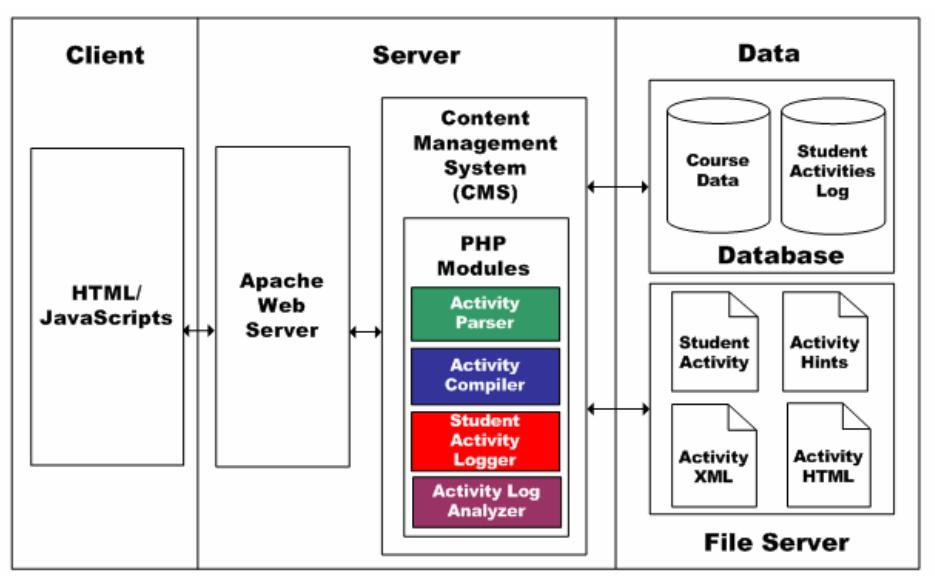
\includegraphics[width=0.9\linewidth, keepaspectratio =
1]{./images/SystemArch01_OUHK_DistanceEdu.jpg}
  \caption{Sistemska arhitektura spletnega portala za učenje
    programiranja, kot so jo naredili na OUHK \cite{ITaLCP_DistanceEdu}.}
  \label{fig:OUHK_cmsArch}
\end{figure}

Ti moduli so naslednji, zajem aktivnosti, prevajalnik aktivnosti,
dnevnik študentove aktivnosti in analizator dnevnikov aktivnosti. Samo
delovanje je naslednje, ko odjemalec pošlje zahtevo za neko aktivnost,
se ta naslovi strežniku, ki poišče programsko aktivnost. Z modulom
\emph{zajema aktivnosti}, strežnik zajame aktivnost, ki je zapisana v
obliki \textbf{XML} in naloži vse potrebne datoteke. Zajem aktivnosti,
prav tako naloži študentovo predhodno delo, ki je shranjeno datoteki
aktivnosti. Ko se vse zajame in naloži se vsebina pošlje v obliki
\textbf{HTML} nazaj k klientu.

Strežnik omogoča tudi prevajanje aktivnosti. Ko strežnik dobi prošnjo
za prevajanje programske kode, se ta prevede, če seveda v njej ni
sintaktičnih napak in se ustvari datoteka \textbf{JAR}, ki jo študent
lahko prenese s strežnika. Če so v programu napake, se ustvari dnevnik
napake, v trenutni aktivnosti, prav tako se napaka izpiše na zaslonu
študenta. Vsako aktivnost zajame dnevnik študentove aktivnosti in jo shrani v
podatkovno bazo. Z analizatorjem dnevnika študentove aktivnosti,
mentorji dobijo vpogled v delo študenta in njegovega napredka.


\subsection{Pregled delovanja in interakcija s SPUP}
\label{sec:pregled_delovanja_in_interakcija}

V nadaljevanju opišimo, kako so si zamislili interakcijo med študentom
ne OUHK.  in mentorjev s spletnim sistemom, diagram prikazuje slika
\ref{fig:OUHK_workFlow}. Spletni sistem omogoča študentom in mentorjem
spletno okolje za učenje programiran. Mentorji na spletni portal
naložijo snov preko spletnega brskalnika. Mentor lahko naloži datoteke
opisom aktivnosti. Ta datoteka vsebuje osnovne opise in informacije o
aktivnostih. Posebej naloži še datoteko v kateri je predloga za
aktivnost. V to predlogo študent rešuje zadano nalogo. V posebno
datoteko je naložen tudi namig, ta je študentu v pomoč in ponuja
primer izpisa programa.

\begin{figure}[htb!] \centering
  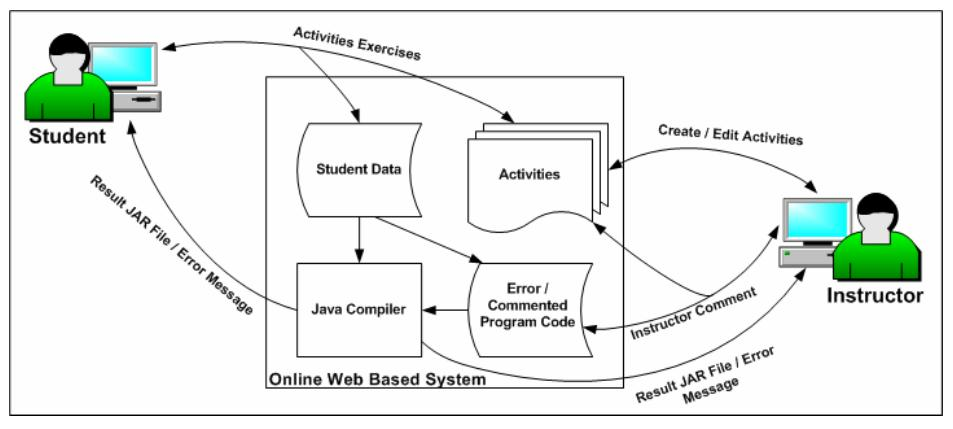
\includegraphics[width=0.9\linewidth, keepaspectratio =
1]{./images/SystemArch02_OUHK_DistanceEdu.jpg}
\caption{Prikaz med interakcijo študenta in mentorja s spletnim
  portalom \cite{ITaLCP_DistanceEdu}.}
  \label{fig:OUHK_workFlow}
\end{figure}

Študent lahko pregleduje vse aktivnosti in si naloži katero koli izmed
njih. Omogočeno ima, da program prevede na strežniku, ko prevajalnik
naleti na napake strežnih vrne napako na spletno stran. Če študent
naleti na težavo, ki je povezana z reševanjem aktivnosti, lahko pošlje
prošnjo za pomoč svojemu mentorju. Ko se mentor prijavi v sistem ima
vpogled v napako in na začasno delovno datoteko študenta, mentor lahko
zaganja prevajalnik na tem začasnem projektu študenta. Ko mentor
popravi programsko napako, odgovori študentu in poda komentar na
programsko kodo študenta. Študent ima vpogled v komentarje in
predloge, ki jih je posredoval mentor \cite{ITaLCP_DistanceEdu}.

%%NJihova diskusija, zaključek in nadaljnjo delo.

Na univerzi v US \cite{mentalModels}, je okrog strategije kognitivnega konflikta
nastalo spletno okolje, ki naj bi izboljšalo mentalne
modele ključnih programskih konceptov. Učni model je sestavljen iz
štirih korakov:

\begin{itemize}
\item \textbf{Predhodni korak:} Mentor razišče kakšni so predhodni
 mentalni modeli študentov in identificira neprimerne.
\item \textbf{Korak kognitivnega konflikta:} V študentovi predstavi
  moramo sprožiti tak dogodek, ki v študentu izove neskladje z njegovo
  predhodno predstavo in s tem študenta potisnemo v konfliktno
  situacijo.
\item \textbf{Korak konstruiranja modela:} Študentu s pomočjo
  visualizacije pomagamo ustvariti pravo mentalno predstavo.
\item \textbf{Korak aplikacije: } Študent mora rešiti programsko
  nalogo z na novo ustvarjeno mentalno predstavo.
\end{itemize}

V nadaljevanju bomo pregledali na kakšen način so si uporabo spletnega
okolja zamislili.  Spletno učno okolje podpira programski jezik
\textbf{JAVA}. Za učenje programskih konceptov je na spletni strani
vsak posamezen koncept povezan z potjo, ki predstavlja načrt
potovanja. Poti koncepte se povezujejo tako, da se ti nadgrajujejo,
saj znanje določenega koncepta potrebuje neko predznanje
prejšnjega. Tako za razumevanje določevanja reference najprej
potrebujemo predznanje o spremenljivkah ali npr. preden se študenti
učijo kako s podajajo parametri v podprograme najprej morajo razumeti
kaj je obseg nekega pod programa. Torej je vrstni red spoznavanja
programskih konceptov pomemben. Med potmi so gumbi, ki predstavljajo
vsak koncept. Na vsakem gumbu je označen rdeč križ kar pomeni, da
študent še ni spoznal koncepta. Ko študent opravi naloge povezane s
posameznim konceptom se rdeč križ spremeni v zeleno kljukico. Ko
študent vstopi v koncept se izpiše študentova zgodovina z nalogami
tega koncepta. Vsaka naloga vsebuje tako vprašanje, ki sproži
konfliktno situacijo v mentalnem modelu študenta. Nato študenti dobijo
učni material v visualni obliki. Za vizualizacijo uporabljajo orodje
\href{https://cs.joensuu.fi/jeliot/}{\textbf{Jeliot}}, ki dinamično
upodablja izvajanje javaskih programov. Za pravilnost razumevanje
mentalnega modela mora študent odgovoriti na dodatna vprašanja. Če
študentovi odgovori niso v skladu z podanim mentalnim modelom, dobi
študent povratno informacijo o nepravilnem odgovoru. Naslednji korak
je ta, da študent mora zagnati vizualizavijo dela programske kode, ki
si ga je prej moral predstavljati. Tako ima možnost, da zazna
nepravilnost v svojem mišljenju in tako lahko gradi na pravilnem
konceptu \cite{mentalModels}.

Poglejmo primer spletnega portala, ki ga je izdelal avtor
\cite{thesisAWebP}, in ima naslednje elemente.

\begin{enumerate}
%\def\labelenumi{\arabic{enumi}.}
\tightlist
\item
  Spletni portal za programiranja, ki omogoča naloge tipa ``Zapolni
  prazna mesta''.
\item
  Ogrodje za analizo, ki preverja kvaliteto in pravilnost, nalog, tipa
  ``Zapolni prazna mesta''.
\item
  Avtomatski sistem za dajanje povratnih informacij, ki sporoča
  prilagojena sporočila prevajalnika in formalni odziv študentom in
  njihovim mentorjem. Poročilo vsebuje kvaliteto napisanega programa,
  strukturo in pravilnost glede na programsko analizo.
\end{enumerate}

%\subsubsection{Analiza programske kode}
%\label{sec:analiza_programske_kode}

% Različne vrste analiz in povratna informacije o napakah. Kako je to
% dobro urejeno pri spletnih portalih*?

Dober odziv spletnega portala mora dati poročilo o pravilnosti programa in o
kvaliteti \cite{thesisAWebP}.

Ogrodje (ang. framework) za analizo programske kode naj bi vsebovalo:

\begin{itemize}
\tightlist
\item
  Sintaktično ali semantično opozarjanje na napake ali napake
  prevajalnika
\item
  odziv na kvaliteto in pravilnost programske kode //Ali ga sistem nima
  ali je ta pomnanjlkjiv. //Zgornje pomaga predvsem slabpim učencem.
  //Večina sistemov izvaja statično analizo programske kode in tako ni v
  pomoč kakšne kvalitete je ta koda.
\item
  Formalni odzin učitelja oz. komunikacija med učiteljem in učencem.
\end{itemize}



\subsection{Rezultati izvedenih rešitev SPUP}
\label{sec:rezultati_izvedenih_rešitev}

Večina študentov smeri računalništva na OUHK nima predhodnih izkušenj
v programiranju z programskim jezikom \textbf{JAVA}. Sistem se
uporablja kot spletno okolje za učenje programiranja. Študentom je s
tem, dana množica aktivnosti oz. nalog, katere morajo sami uspešno
opraviti. To lahko počnejo kadarkoli in od koderkoli. Študentom ni
potrebno nastavljati programskega okolja, študenti vse programe, ki
jih napišejo, lahko takoj prevedejo in jih zaganjajo na svojih
računalnikih. Uporaba spletnega portala je pokazala da so študentje
oddali 100\% programskih nalog, napisanih v javi. To kaže na to, da so
študentje samozavestno reševali naloge in jih oddajali. Pred uporabo
spletnega portala je oddaja nalog bila 80\%.

Kot pravijo avtorji članka in portala \cite{ITaLCP_DistanceEdu}, je to
šele začetek uporabe spletnega portala, ki nudi osnovno
funkcionalnost. V nadaljevanju nameravajo dodati še inteligentni
sistem, ki po nadzoroval napredek študentov.

Za izboljšanje mentalnih modelov so avtorji predlagajo konstruktivno
naravna učni model, ki vključuje strategijo kognitivnega konflikta in
vizualiacijo programov. Zgodnje preizkušanje strategije kognitivnega
konflikta pokažejo da so študenti bolj zavzeti za učni material in jih
motivira tako, da si prej ustvarijo pravilno mentalno predstavo
\cite{mentalModels}.

%%Učno okolje.
%%Preglej pravilnost programerskih slovenskih izrazov.
%% Slika portala za članka.


Nekatere osnove težave, katere srečajo programerji novinci \cite{thesisAWebP}:
\begin{enumerate}
\tightlist
\item
  Inštalacija in nastavitve okolja za programiranje.
\item
  Uporaba urejevalnika besedil.
\item Razumevanje napisanih nalog oz. problemov in uporabe sintakse
  programskega jezika pri pisanju programske kode.
\item
  Razumevanje napak prevajalnika.
\item
  Razhroščevanje.
\end{enumerate}

V preteklosti je bilo razvitih mnogo orodij, ki so nastala ravno z
raziskovanja učenja programiranja, vendar mnoga od teh zahtevajo, da
študenti pišejo celotne programe od začetka do konca.

Tudi začetniki, ki uspešno premagajo začetne ovire in se lotijo
takojšnjega programiranja, imajo zelo slabo napisano in konstruirano
programsko kodo. Pomagati novincem, pistati kvalitetno programsko kodo
je časovno zelo zahtevno opravilo.

%Danes se večini uči OO jezikov, kako podkrepiti to tezo.
Težave programiranja se stopnjujejo ko se za učenje programiranja
uporabljajo Objektno-orjentirani programski jeziki, sej ti zahtevajo
visoko stopnjo abstraktnega razumevanja programskih konceptov in so
načrtovani predvsem za zahtevne programerje.

% Torej je pomembno v katerih programskih jezikih se začnemo učiti
% programiranja? Zakaj sta zato primerna? -> Scratch in Python?  Kje
% je določeno na državnem nivoju da se učit ravno ta dva programska
% jezika



\subsection{Povzetek problematika začetkov učenja programiranja}
\label{sec:Problematika_začetkov_učenja_programiranja}

% Po pregledu, ki se ukvarjajo z učenjem programiranja lahko
% ugotovimo, da je samo učenje programiranja tanko staro kot prvi
% program, ki je bil kdaj koli napisan.

% NOTE: Razlikovati moramo med kodiranjem in reševanjem problemov
% Začetne misli o učenju programiranja.

% NOTE: Zanima nas naslednja vprašanja:
% NOTE: * Kaj so spletni portali za učenje programiranja?
% NOTE: * Zakaj in kje je smiselno uporabljati spletne portale za
% NOTE:   učenje programiranja.
% NOTE: * Prednosti spletnih portalov in slabosti?
% NOTE: * Kako so spletni portali zgrajeni?
% NOTE: * Katere so različne vrste spletnih portalov (Kategorije) in
% NOTE:   katere bodo nas zanimale?
% NOTE: *

% Kateri tradicionalni spletni portali? Preveri?
% Ali že tu pisati, da v tem primeru gre za učenje na daljavo?!
Tradicionalni spletni portali v izobraževanju, kot so \textbf{moodle},
nikoli niso popolnoma izkoristili zmožnosti uporabe, ki jih ponujajo
nove internetne in komunikacijske tehnologije. Večinoma so se
uporabljale le kot podaljšana roka obstoječim metodam
poučevanja. Uporabljale so se za objavo gradiv in spletno prijavo za
oddajo nalog. Takšni sistemi ne zagotavljajo izboljšav kvalitete
poučevanja programiranja \cite{ITaLCP_DistanceEdu}.

Strnimo nekatere značilnosti težav novincev.

\begin{itemize}
\tightlist
\item Težave pri namestitvi in nastavitvah programske opreme,
  prevajalnika in razvojnega okolja (OUHK, ).
\item Dostop do mentorjev zaradi časovne dostopnosti in Komunikacija v
  primeru izobraževanja na daljavo (OUHK).
\item
\end{itemize}

V začetku nas bo zanimalo kaj so spletni portali za učenje. Spoznali
bomo, da poznamo različne kategorije spletnih portalov za posredovanje
različnega znanja in veščin. Zanimali nas bodo  predvsem spletni
portali, ki učijo znanje programiranja.
%Posvetili se bomo predvsem takšnim in podobnim spletnim portalom!

\subsection{Predlagane rešitve SPZUP na težave novincev}
\label{predlagane_rešitve_na_težave_novincev}

Pri samem vadenju programiranja je pomembno, da ob težavah, novinci
dobijo čimprajšen odziv mentorja. V velikih razredih se to izkaže za
zelo zahtevno. Z uporabo spletnih tehnologij so v pomoč prav spletni
portali za učenje programiranja. Z njimi lahko razrešimo kar nekaj
tegob, ki jih pestijo novince \cite{thesisAWebP}.

Ena od prednosti dela z takšnim sistemom je ta, da novinci niso odvisni
od mentorjevih uradnih govorilnih ur, pravtako tako lahko naloge
opravljajo kadar koli \cite{thesisAWebP}.

\section{Strategije reševanja problemov}
\label{sec:strategije_reševanja_problemov}

Programiranje je preces pri katerem rešujemo probleme. Reševanje
problemov, zato mora biti središče poučevanja računalniške
znanosti. Reševanje problemov je zahteven mentalni proces. Če na
spletu pobrskamo za strategije reševanja problemov lahko hitro
ugotovimo na obstajajo različne strategije. Kot so recimo naštete na
strani
\href{https://en.wikipedia.org/wiki/Problem_solving#Problem-solving_strategies}{Wikipedia:Reševanje
  problemov (\emph{ang. Problem solving})}, abstrakcija, analogija,
brainstorming, deli in vladaj in mnoge druge.  Proces in tehnike
reševanje problemov se uporablja v mnogih tehničnih in znanstvenih
disciplinah \cite{guideTCS}.

V nekaterih primerih učenci sami razvijejo strategijo s katero rešijo
nek problem. Otroci si na primer sami izmislijo enostvno seštevanje in
odštevanje, dolgo pred tem kadar se to učijo pri pouku
matematike. Toda brez formalne podpore za unčikovito strategijo
reševanja problemov, spodleti še tako inovativnemu učencu tudi pri
enostavnih strategijah kot je \textbf{preizkus in napaka}. Zato je
pomembno, da se uči strategij za reševanje problemov.

\subsection{Proces reševanja problemov}
\label{sec:proces_reševanja_problemov}

Vsak osnoven proces, ki se ukvarja z raševanjem problemov, ne glede na
znanstveno disciplino, se začne z opisom problema. Vsak problem se
navadno zaključi z neko rešitvijo, ki je v nekaterih primerih izražena
z \textbf{zaporedjem korakov} ali \textbf{algoritmom}. V računalništve
algoritem zapišemo z kodo nekega programskega jezika. Zapisan
algoritem testiramo tako, da kodo zaženemo, jo izvedemo. Preden
pridemo od opisa problema do podane rešitve moramo prehoditi kar nekaj
težkih korakov. Na te vmesne korake lahko gledamo kot na procese
odkrivanja, zato lahko na reševanje problemov gledamo tudi kot na
kreativen, umetniški proces \cite{guideTCS}.

Splošno priznani koraki reševanja procesov so naslednji:

\begin{enumerate}
\tightlist
\item \emph{Analiza problema}. Najprej je pomembno da razuemo kaj je
  problem in ga znamo identificirati. Če tega ne znamo, ne moremo
  priti do nobene rešitve.
\item \emph{Alternativnie rešitve}. Razmišljamo o alternativnih
  rešitvah kako bi lahko rešili nek problem.
\item \emph{Izbira pristopa}. Izberemo primeren pristop, kako rešiti problem.
\item \emph{Razgradnja problema}. Problem razgradimo na manjše podprobleme.
\item \emph{Razvoj algoritma}. Algoritem razvijamo po korakih, ki smo
  jih določili v podproblemih.
\item \emph{Pravilnost algoritma}. Preverjanje pravilnosti algoritma.
\item \emph{Učinkovitost algoritma}. Izračunamo učinkovitost algoritma.
\item \emph{Refleksija}. Naredimo refleksijo in analizo na pot, ki smo
  jo naredili pri reševanju problema in naredimo zaključek z tem kar
  lahko izboljšamo za naslednji problem, ki ga bomo reševali.
\end{enumerate}

Točen recept kako se lotiti reševanja ne obstaja. Učencem lahko le
pokažemo nekatere metode in strategije, ki jim lahko pomagajo pri
reševanju problemov. Poglejmo še nekatere pomembne korake podrobneje.

\subsubsection{Razumevaje problema}
\label{sec:razumevanje problema}

Razumevanje problemov je prva stopnja v procesu reševanja
problemov. Pri reševanju algoritemskih nalog najprej moramo
prepoznati, kaj so vhodni podatki in kateri podatki naj bi bili
izhodni. Če znamo povedati kaj bodo vhodni podatki, razumemo tudi
bistvo samega problema.

\subsubsection{Načrtovanje rešitve}
\label{sec:načrtovanje_rešitve}

Novinci se spopadajo z največjimi težavami na začetni stopnji
načrtovanja rešitve za nek problem. V nadaljevanju so predstavljene
tri strategije, ki jih lahko uporabimo na tem koraku reševanja
problema.

\begin{description}
\item [Definicija spremenljivk problema:] Pri rešitvi problema
  si pomagamo tako, da ugotovimo kaj morajo biti vhodni in kateri bojo
  izhodni podatki. S tem razjasnimo problem. V naslednjem koraku
  definiramo \textbf{spremenljivke}, ki so potrebne za rešitev
  problema.
\item [Postopno izboljševanje (\emph{ang. Stepwise
      Refinement)}:]Po tej metodi nas najprej zanima celoten pregled
  strukture problema in odnosi med posameznimi deli. Zatem se šele
  poglobimo specifični in kompleksni implementaciji posameznih pod
  problemov. Postopno izboljševanje je metodologija, ki poteka od
  \textbf{zgoraj-navzdol}, torej od splošnega k specifičnemu. Drugačen
  pristop je od \textbf{spodaj-navzgor}. Za oba pristopa velja da eden
  drugega dopolnjujeta. V obeh primerih je problem razdeljen na manjše
  pod probleme ali naloge. Glavna razlika med obema je mentalni
  proces, ki je potreben za en ali drugi pristop.  V nadaljevanju se
  posvetimo samo pristopu od \textbf{zgoraj-navzdol}. Rešitev, ki jo
  poda \textbf{postopno izboljševanje} ima modularno obliko, ki jo:
  \begin{enumerate}
    \tightlist
  \item jo lažje razvijamo in preverjamo,
  \item jo lažje beremo in
  \item nam omogoča, da uporabljamo posamezne pod rešitve tudi za
    reševanje drugih problemov.
  \end{enumerate}
\item [Algoritemski vzorci:] Algoritemski vzorci združujejo
  matematični pogled in elemente načrtovanja. Vzorec podaja načrt na
  rešitev, s katero se srečamo mnogokrat. Algoritemski vzorci so
  primeri elegantnih in učinkovitih rešitev problemov in predstavljajo
  abstraktni model algoritemskega procesa, katerega lahko prilagodimo
  in ga integriramo v rešitve drugim problemom.

  Pri tem procesu lahko nastopi težava prepoznave vzorca algoritma pri
  novincih, saj ti niso sposobni prepoznati podobnosti med posameznimi
  algoritmi ali ne znajo prepoznati bistvo problema, njihove posamezne
  komponente in razmerja med njimi, da bi lahko rešili nove
  probleme. V takih primerih novinci radi ponovno izumijo že njim
  poznane rešitve, ki bi jih lahko uporabili. Te težave navadno
  nastanejo zaradi slabe organizacije sistematike znanja o algoritmih.

  Proces reševanja problemov z algoritemskim vzorcem se navadno začne
  z prepoznavanjem komponent, ki vodijo k rešitvi in iskanjem podobnih
  problemov, na katere še imamo znane rešitve. Zatem prilagodimo
  vzorec prilagodimo za rešitev problema in ga vstavimo v celotno
  rešitev. V večini primerov je potrebno vstaviti več različnih
  vzorcev, da dobimo neko novo rešitev.
\end{description}

\subsubsection{Preverjanje rešitve}
\label{sec:preverjanje_rešitve}
Ko imamo pripravljeno rešitev moramo preveriti ali je ta
pravilna. Pogled na preverjanje pravilnosti rešitve je lahko
teoretične in praktične narave. Razhroščevanje (\emph{ang. debugging})
spada me vrsto aktivnosti, ki nam pomaga pri ugotavljanju pravilnosti
rešitve. Splošno velja da proces razhroščevanja, z programom, ki nam
pomaga razhroščevati (ang. debugger) ali brez njega, poglablja
razumevanje računalniške znanosti. Z tem ko učenci razmišljajo, kako
bodo preverjali ali njihov program deluje pravilno, hkrati v njih
poteka miselni proces refleksije o tem kako so implementirali določen
program in kako ga bojo morebiti morali spremeniti.

Na nivoju do srednje šole uporabljamo praktične metode ugotavljanja
pravilnosti programa, kot je razgroščevanje. Ko želimo znanje
pravilnosti delovanja poglobiti se lahko lotimo tudi teoretične
analize.

\subsubsection{Refleksija}
\label{sec:refleksije}

Refleksija je mentalni proces ali obnašanje, ki nam omogoča da neko
delovanje analiziramo in o njem tudi premislimo. Refleksija je
pomembno orodje v splošnem učnem procesu, prav tako spadam med
kognitivne procese višjega reda. Z refleksijo učenec dobi priložnost,
da stopi korak nižje in premisli o svojem razmišljanju in tako
izboljša veščino reševanja problemov. Refleksivno razmišljanje je
proces, ki zahteva veliko časa in vaje. Med procesom reševanja
problemov, lahko refleksijo uporabimo na različnih stopnjah.

\begin{itemize}
\tightlist
\item \emph{Pred} reševanjem problemom. Ko problem preberemo, in že
  načrtujemo rešitev, se splača uporabiti refleksijo in razmisliti o
  tem ali smo morda že reševali podoben problem in temu primeren
  vzorec algoritma.
\item \emph{Med} reševanjem problema. Ko rešujemo problem refleksija
  služi, kot pregled, kontrola in nadzor. Na primer, ko nastopijo
  težave pri načrtovanju rešitve ali morda zaznamo težavo ali
  napako. Temo procesu lahko pravimo \textbf{refleksija v akciji}.
\item \emph{Po} reševanju problema. Ko že najdemo rešitev, ki deluje,
  nam refleksija služi kot orodje z katerim pregledamo učinkovitost
  delovanja. Pregledamo strateške odločitve, ki so bile sprejete med
  samim načrtovanjem rešitve.
\end{itemize}

Refleksija je kreativni proces in je pomemben za učenca tako kot za
učitelja.

\section{Metode in strategije pri uporabi spletnih portalov}
\label{sec:Metode_in_strategije_pri_učenju_programiranja}

Primer strategij in metod spletnega portala za učenje \textbf{Jave}.
\cite{thesisAWebP}:

\begin{itemize}
\tightlist
\item
  Scaffolding -\textgreater{} Gradnja študentovega znanja
  pri katerem pomaga mentorja, z svojim znanjem in izkušnjami.
\item
  Bloomova taskonomija. Zakaj je pomembno vključevanje Bloomove
  taksonomije in kako jo vključujemo.
\item
  Konstruktivizem: Aktivnost študentov pri gradnji znanja. Učenje z
  eksperimentiranjem. Problemski pristop.
\end{itemize}

Kaj od katerih metod predstavlja v uporabi spletnega portala \ldots{}:

\begin{itemize}
\tightlist
\item
  Spletni portal -\textgreater{} Scaffolding + Bloom
\item
  Naloge narejene tako, da podpirajo konstrutivno metoIn tudi nekatere slabosti, če hih najdem v literaturi
  -\textgreater{} problemski pristopom
\end{itemize}

V naslednjem poglavju sledi pregled tehnik aktivnih metod
poučevanja. V poglavju sledi obravnava didaktičnih pripomočkov, oblik
pouka, in projektno delo \cite{guideTCS}.
\subsection{Didaktični pripomočki}
\label{sec:didaktični_pripomočki}

Med didaktičnimi pripomočki najdemo številna orodja:

\begin{itemize}
\tightlist
\item \textbf{pedagoške igre},
\item računalništvo brez računalništva,
\item \textbf{bogate naloge},
\item miselni vzorci,
\item klasifikacija,
\item metafore.
\end{itemize}

V povezavi z spletnimi portali za učenje programiranja nas bodo
zanimale le nekatera.

\subsubsection{Pedagoške igre}
\label{sec:pedagoške_igre}

\subsubsection{Bogate naloge}
\label{sec:bogate_naloge}

\subsection{Različne organizacijske oblike pouka}
\label{sec:različne_oblike_pouka}

Računalniško znanost lahko poučujemo tako, da jo predavamo, vendar to
ni v skladu z naprednimi nazori poučevanja aktivnega učenja, ki smo ga
do sedaj spoznali. Za uspešno in koristno učenje se moramo temu
pristopu čim bolj izogniti. To velja predvsem za izobraževanje na
nivoju \textbf{OŠ} in seveda tudi \textbf{SŠ}. Kot smo že poudarili v
poglavju? je pomemben aktivni pristop v učnem procesu.

Pomembno je tudi v kakšni obliki dela poteka pouk. V nasprotju z
frontalnim delom, lahko pouk organiziramo na naslednje načine.

\begin{description}
\item[Samostojno delo:] Prvi način je morda najenostavnejši
  za organizacijo dela v učilnici in omogoča aktivno učenje za vse
  učence. Taka oblika organizacije je primerna predvsem, ko učitelj
  želi preveriti ali vsi učenci sledijo in znajo uporabljati določeno
  znanje in veščine, kot je na primer uporaba integriranega razvojnega
  okolja (\emph{ang. Integrated Development Environment
    +(\textbf{IDE})}) ali sledenje določenemu algoritmu.
\item[Delo v parih:] Razred razdelimo v pare, ti rešujejo
  programerske ali ne programerske naloge. V primeru programerskih
  nalog, učenca, ki sta v paru rešujeta programersko nalogo tako da je
  eden v vlogi \textbf{voznika} in drugi v vlogi
  \textbf{navigatorja}. Prvi, voznik ima v nadzoru tipkovnico in
  miško. Drugi sledi razvojnemu procesu in analizira napredek skupaj z
  voznikom. Oba seveda zamenjujeta vloge. Programiranje v parih vodi v
  proces reševanja problemov na dveh nivojih, en nivo predstavlja
  nalogo kodiranja, drugi predstavlja uporabo strategij pri reševanju
  problema. Ko so naloge niso programerske in jih ne izvajamo na
  računalniku, zgubimo nalogo voznika. Kljub temu lahko izvajamo tako
  obliko pouka, saj lahko sklepamo, da je delo v parih, pri reševanju
  problemov, primernejše kot v večjih skupinah, kjer obstaja večja
  možnost, da nekateri učenci dominirajo v skupini in teko druge
  učence prikrajšajo za sodelovanje.
\item[Skupinsko delo] Druga oblika organizacije je delo v
  skupi ali timu in je primerna v naslednjih primerih:
  \begin{enumerate}[a.]
  \item ko sta potrebna več kot dva učenca za opravilo neke naloge,
  \item Ko učitelj želi izkoristiti raznolikost v skupini,
  \item ko je razred razmeroma velik in si učitelj želi olajšati delo
    tako da učence razdeli v manjše skupine,
  \item ko želi da so vključeni vsi učenci, a le eden iz posamezne
    skupine naj bi predstavljal narejeno delo.
  \end{enumerate}
\item[Skupinsko delo - sestavljanka (\emph{ang. Jigsaw Classroom})] Po
  navodilih spletne strani \href{https://www.jigsaw.org/}{razredne
    sestavljanke (\emph{ang. Jigsaw classroom})} je oblika
  organizacije na naslednji način.
  \begin{enumerate}
  \item Učence razdelimo na skupine 5 - 6. Vsak od njih ima nalogo, da
    predela posamezno nalogo, poglavje, ki je razdeljeno na toliko pod
    poglavij ko je učencev v skupini. Vsak od njih je odgovoren, da se
    nauči posamezno podpoglavje in to znanje posreduje naprej drugim
    učencem.
  \item Preden učenci preidejo k poročanju posameznega podpoglavja, se
    sestanejo z učenci drugih skupin, ki imajo isto nalogo oz
    podpoglavje. S tem zagotovimo večjo točnost naučenega.
  \item Učenci se vrnejo nazaj v svoje prvotne heterogene skupine, in
    poučijo svoje sošolce o tem kaj so se naučili.
  \end{enumerate}
  Učitelj se odloči kaj po končni izdelek, ali bo to napisano kratko
  poročilo, ali plakat, ali kak drugi pisni izdelek, delo se lahko
  zaključi tudi brez končnega izdelka.

  Kot je razvidno z organizacije dela \textbf{sestavljanke} so
  prednosti ogromne, tiste ki omogočajo kognitivni razvoj in tiste, ki
  socialnega. Učenje v tej obliki vzpodbuja učenje, poslušanje,
  sodelovanje in deljenje znanja.
\end{description}

\subsection{Programirana pouk}
\label{programirani_pouk
}



\subsection{Projektno delo}
\label{sec:projektno_delo}

Preglejmo najprej nekatere lastnosti, ki jih prinaša projektno
delo. To lahko poteka tako, da učenci delajo samostojno ali v
skupini. Učitelj je tisti, ki vodi proces projektnega dela. Učenec je
pri projektnem delu bistveni člen in mu tako omogoča aktivno učenje.

\subsection{Učne strategije}
\label{sec:učne_strategije}

\subsubsection{Aktivno učenje in model aktivnega učenja}
\label{sec:aktivno_učenje_in_model_aktivnega_učenja}

Vsak pouk računalništva mora biti zgrajen kot model in bi moral
upoštevati naslednja načela:
\begin{itemize}
\tightlist
\item Vzpodbujati mora študente z pozitivno naravnanim poukum in
   omogočati mora okolje kjer študent najde pomoč.
 \item Pouk računalništva je grajen na konstruktivnih metodah poučevanja
   in aktivnem učenju.
\end{itemize}

\textbf{Konstruktivizem} je kognitivna teorija, ki preučuje naravo
procesov učenja. Po tem principu naj bi učenci konstruirali novo
znanje na osnovi preurejanja in izpopolnjevanja že obstoječega
znanja. Znanje se gradi na obstoječih mentalnih strukturah in na
odzivu, ki ga dobi učenec iz učnega okolja. Mentalne strukture so
grajene korak za korakom, ena za drugo, seveda s to metodo lahko pride
tudi do sestopanja ali slepih koncev. Proces je povezan z Piagetovim
mehanizmom asimilacije \cite{guideTCS}.

Pri \textbf{aktivnem učenju} je najpomembnejše to, da učenci z lastno
aktivnostjo ugotovijo, sami za sebe kako nekaj deluje. Sami si morajo
izmisliti primere, preiskusiti lastne veščine in reševati neloge, ki
so jih že ali jih še podo spoznali. Učenje je aktivno usvajanje, je
gradnja idej in znanja. Za učenje mora biti posameznik aktivno
vključen v gradnjo svojih lastnih mentalnih modelov.

Model aktivnega učenja je sestavljen s štirih korakov \cite{guideTCS}.

\begin{itemize}
\tightlist
\item \textbf{Sprožilec} Je je naloga, ki predstavlja  iziv za uvod v novo
tematiko.  //Gerlič -> Motivacija.
\item \textbf{aktivnost} Študenti izvajajo aktivnost, ki jim je bila
predstavljena v sprožilcu. Ta kora je lahko kratek ali lahko
zavzame večju del učne ure. To je odviso od vrste sprožilca in
izobraževalnih ciljev.
\item \textbf{diskusija} sledi po koncu aktivnosti, kjer se zbere zeloten
razred, neglede na obliko dela. V temo koraku študenti izpopolnijo
koncepte in ideje, kod del konstruktivnega učnega procesa.
\item \textbf{povzetek} je lahko izračen v različnih oblikah, kot so
zaogrožene definicije, lahko so miselni vzorci ali povezav med
temami, ki so jih obravnavali študenti in med drugimi temami, ki se
navezujejo nanje.
\end{itemize}

Ko se ta model izkaže za primernega, ga lahko uporabimo v številnih
učnih urah v različnih variacijah.

\subsubsection{Učenje  na daljavo}
\label{sec:Učenje_na_daljavo}


\subsection{Tipi nalog}
\label{tipi_nalog}

\subsubsection{Zapolni prazna mesta}
\label{sec:zapolni_prazna_mesta}

Tip nalog začetniku ponuja ogrodje programa, del programske kode, na
katerem dijak usvoji novo znanje in/ali lahko uporablja že pridobljeno
znanje.


\section{Kategoriziranje spletnih portalov}
\label{sec:kategoriziranje_spletnih_portalov}

\subsection{Vrsta vsebine}
\label{sec:Razvrstitev_spletnih_portalov}

Po hitrem pregledu izbranih spletnih portalov lahko ugotovimo, da je

\subsection{Programski jeziki}
\label{sec:programski_jeziki}


\section{Ovrednotenje izbranih spletnih portalov in njihove posebnosti}
\label{sec:pregled_spletnih_portalov}

\subsection{Pogoji za ožji izbor spletnih portalov}
\label{sec:pogoji_za_ožji_izbor_sp}



\subsection{Določitev Kriterijev}
\label{sec:dolocitev_kriterijev}

Pri vrednotenju spletnih portalov bomo upoštevali naslednje
kriterije,

%Zaenkrat samo povzeto, to kar sem spoznal do sedaj.

\begin{itemize}
\tightlist
\item število programskih jezikov,
\item zahtevano predznanje uporabnika,
\item interaktivna povratna informacija,
\item problemski pristop,
\item jezik spletne strani.
\end{itemize}

\section{Možni načini uporabe spletnih portalov pri pouku}
\label{sec:načini_uporabe_sp},
